\documentclass[../main]{subfiles}

\begin{document}

\chapter{The Scratch programming environment}\label{ch:scratch-the-programming-environment}

%\dictum[S. Papert \\ \textit{Mindstorms}]{In teaching the computer how to think, children embark on an exploration about how they themselves think.}

This chapter is a short introduction to Scratch, both the programming language and the environment.
It also explains how the source code for Scratch is organized.
The main goal is to familiarize the reader with the Scratch environment.
Technical details are given in later chapters where relevant.

\section{The Scratch environment}\label{sec:scratch-environment}

Scratch is a visual programming language and environment~\autocite{resnickScratchProgrammingAll2009}.\footnote{\url{https://scratch.mit.edu}}
Visual programming languages let programmers construct programs by graphically manipulating program elements, rather than textually~\autocite{kelleherLoweringBarriersProgramming2005}.
A subset of visual programming languages are block-based languages, in which programs consist of blocks that are clicked together, not unlike puzzle pieces or Lego bricks~\autocite{weintropBlockNotBlock2015}.
Scratch falls in the category: it consists of a set of blocks with different shapes and colours.
Development on it began in 2002, by the Lifelong Kindergarten research group at the MIT Media Lab.
Scratch became publicly available in 2007 and has been developed by the Scratch Foundation since 2009.
Its target audience is young learners, ages 8 to 16, although it is most commonly used for ages 10 to 14.
It is a widely used programming language: the 2022 annual report of the Scratch Foundation~\autocite{scratchfoundationGrowingGlobalCreative2022} states that there are over 50 million users in the online Scratch community, with 120 million new projects created in 2022.
The official statistics show that in April 2024, there were 1.5 million active monthly users, with about 3.7 million new projects.\footnote{\url{https://scratch.mit.edu/statistics/}}
The same month, the Scratch team announced that a billion projects have been created.\footnote{\url{https://twitter.com/scratch/status/1778814544682295394}}
\makenote*{The TIOBE index is not that useful: it is based on the number of reported results in search engines~\autocite{bunceTIOBENotTIOBE2008,sundarramPleaseStopCiting2022}. For example, it is known that the system is gamed~\autocite{bunceTIOBEIndexBeing2009}.}
The TIOBE index for March 2024 ranks it as the ninth most used programming language~\autocite{tiobeTIOBEIndexMarch2024}.

\begin{figure}
    \begin{wide}
        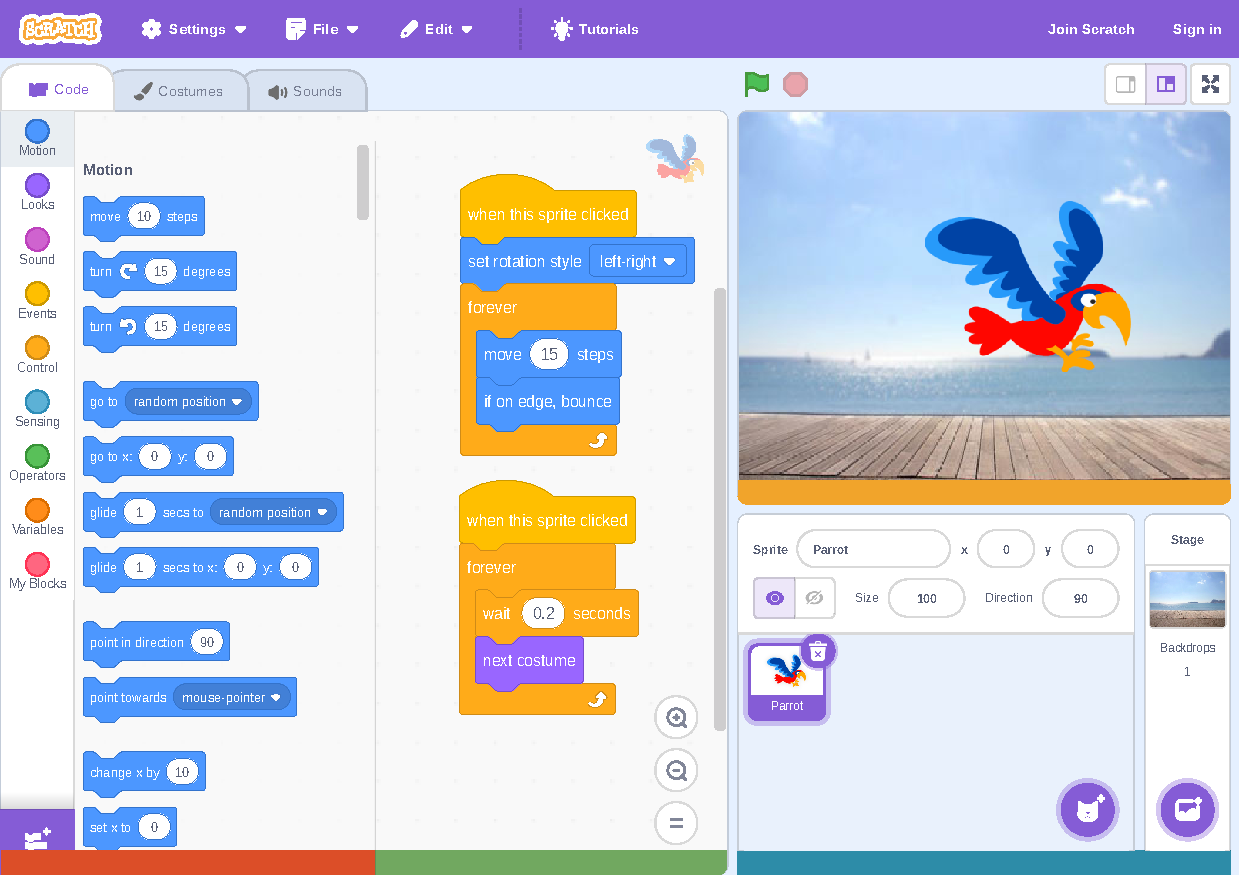
\includegraphics[width=\linewidth]{./scratch-ide}
    \end{wide}
    \caption{The Scratch environment running an example project.
    The toolbox with the available blocks is underlined in \textcolor{ugent-re}{red}, the workspace is underlined in \textcolor{ugent-ps}{green}, the editors for the sprites and the stage are underlined in \textcolor{ugent-we}{blue}, and the canvas is underlined in \textcolor{ugent-lw}{orange}.}
    \label{fig:scratch-environment}
\end{figure}

\subsection{Using the environment and the blocks}\label{subsec:using-the-environment-and-the-blocks}

Blocks can be dragged from the toolbox on the left side of the integrated development environment (\cref{fig:scratch-environment}) to the workspace in the middle and can be stacked together to form scripts.
Blocks are categorized by their subject or goal: \textcolor{scrmove}{Motion}, \textcolor{scrlook}{Looks}, \textcolor{scrsound}{Sound}, \textcolor{screvent}{Events}, \textcolor{scrcontrol}{Control}, \textcolor{scrsensing}{Sensing}, \textcolor{scroperator}{Operators}, \textcolor{scrvariable}{Variables}, and \textcolor{scrmoreblocks}{My Blocks} (not counting extensions).
Each category has its own colour, except for the blocks that handle lists, as these appear in the \textcolor{scrvariable}{Variables} category but have a different colour.

Each script starts with a hat block that defines when the script should execute.
Scripts can be started as a result of a user action or when a certain criterion is met during the execution of a program, for example, when a clone is started or a message is broadcast.
A common way to start scripts is to press the green flag (\scaledflag{0.8}), which has two functions: it will first stop all running threads before starting new threads for all relevant hat blocks.
The red stop button next to the green flag also stops all currently running scripts.
The green flag button has another functionality: when there are active scripts, the button gets a darker background colour, even if those scripts were not started by the green flag.

Blocks (or parts of scripts) can also be run independently by clicking them.
This illustrates that Scratch is always live: once a project has been loaded, the virtual machine is always running.
Sprites can be moved or manipulated by the user at any time, even if scripts are running.

Each script is connected to a sprite.
Sprites are objects that are drawn on the screen.
The bottom right corner of the environment contains an editor for sprites and the background, which is a special sprite called Stage that is present in every Scratch project.
All scripts corresponding to the selected sprite are shown in the workspace (middle).
The canvas in the top right corner of the environment shows the execution of the project.

Besides the tab for the blocks (the ``code''), there are also tabs for the costumes and sounds.
The costumes are the visual representation of the sprite.
While some blocks control which costume is used, the list of possible costumes must be prepared in this tab in advance.
The sound tab is similar, but for sounds instead of costumes.

Finally, users can manage the sprites and stage at the bottom right.
Sprites can be added and removed (even all sprites) by the user.
Similarly, the ``backdrop'' of the stage (which acts as the costume for the stage) can be modified as well.
Note that the stage cannot be removed.

\subsection{Data types}\label{subsec:scratch-data-types}

Scratch has support for three basic data types: strings, booleans, and numbers~\autocite{maloneyScratchProgrammingLanguage2010}.
A different block shape is used for booleans (a mix between rectangle and diamond) and strings/numbers (round oval).
Variables and reporter blocks (which are special blocks that result in some value) can only be inserted boolean slots if the shapes match.
The string/number slots are less strict: if necessary, Scratch will coerce the data into the right type.
Since the reporter blocks can also use operators, they fulfil the role of expressions.

In addition, Scratch also supports lists with their own set of blocks to manipulate them.
Lists can only contain strings or numbers; booleans are cast to strings.

\subsection{Sprites, the object model}\label{subsec:sprites-the-object-model}

Sprites are the Scratch equivalent to objects~\autocite{maloneyScratchProgrammingLanguage2010}.
As all scripts belong to a particular sprite, almost all blocks only work for the current sprite.
Apparently, an earlier version of Scratch had cross-sprite commands, but users found it confusing.
Since Scratch lacks classes and inheritance, \citeauthor{maloneyScratchProgrammingLanguage2010} call it an ``object-based language''.

The strict separation of code between sprites means there is a lot of work needed to make a set of sprites behave the same way.
For example, a firework might need hundreds of sprites to represent the particles.
Creating copies of the sprites by hand quickly becomes tedious.
That is why Scratch has a clone feature: a ``shadow'' sprite is created that shares its code with the original sprite.
While the code is shared, the execution is not: each clone can execute code independently.
A clone is not visible in the sprite overview, only on the canvas.

Variables are normally also limited to the sprite that defined them and are not visible to other sprites.
There is an exception: the variables of the stage are visible to all sprites and could thus be used for inter-sprite communication.

\subsection{Inter-sprite communication}\label{subsec:intersprite-communications}

\textcolor{screvent}{Broadcasts} are the intended way to let sprites communicate with each other.
There are other ways, such as variables (since variables in the stage are global).
However, broadcasts remain the intended way to do inter-sprite communication.
It is a one-to-many broadcasting system~\autocite{maloneyScratchProgrammingLanguage2010}: a broadcast (an arbitrary string) is sent globally and might trigger multiple scripts (even in different sprites).

\subsection{Defining custom blocks with procedures}\label{subsec:defining-custom-blocks-with-procedures}

Scratch allows defining custom blocks, sometimes called procedures.
This allows the user to define blocks that consist of other blocks, similar to procedures in other languages.
Procedures in Scratch can have parameters that can take arguments, which are available as variables to the blocks of the procedure.
Since the custom blocks are procedures and not functions, they do not have return values.

\subsection{Concurrency and parallelism}\label{subsec:parallelism}

Scratch is a highly concurrent language: every script is akin to a thread and can run concurrently to other scripts, even within the same sprite.
The chosen concurrency model of Scratch has a few advantages but also disadvantages, which we discuss in \cref{subsec:execution-of-a-scratch-program}.

Due to JavaScript's single-threaded nature (the language in which Scratch is implemented), the actual execution of a Scratch program will not be in parallel.

\section{Organization of the source code}\label{sec:scratch-internal}

\begin{figure}
    \begin{wide}
        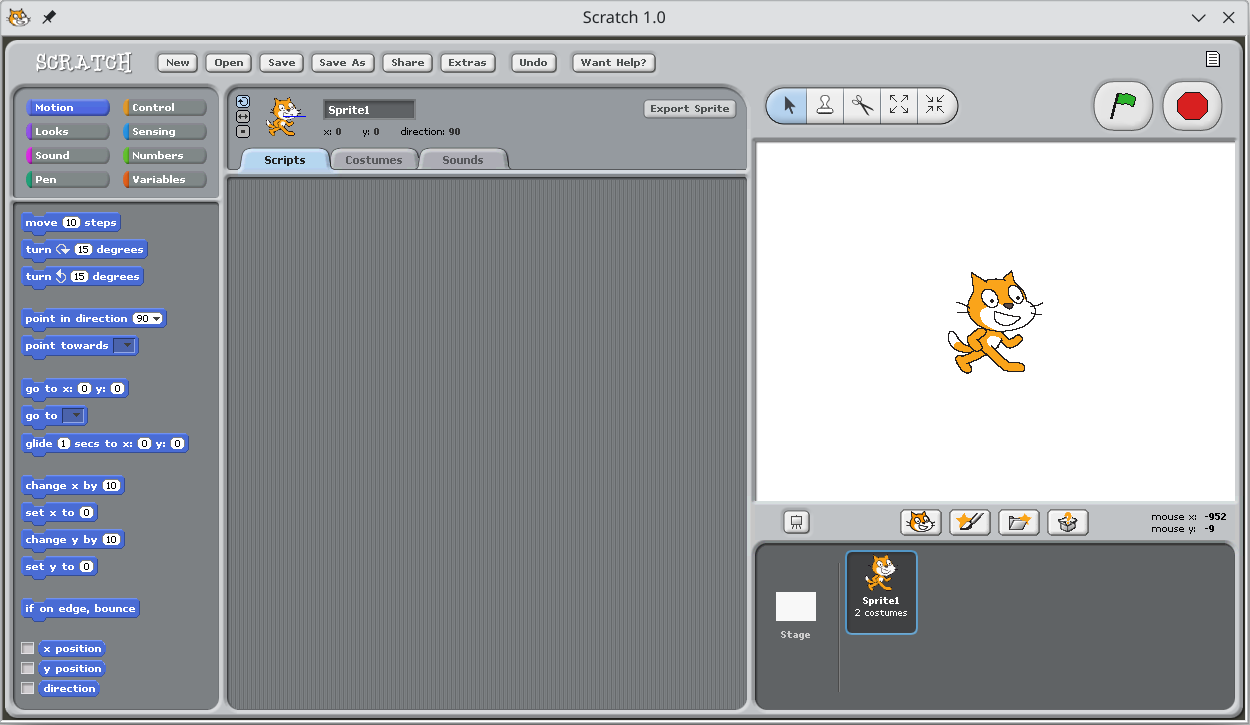
\includegraphics[width=\linewidth]{scratch-1}

        \vspace{0.5em}
        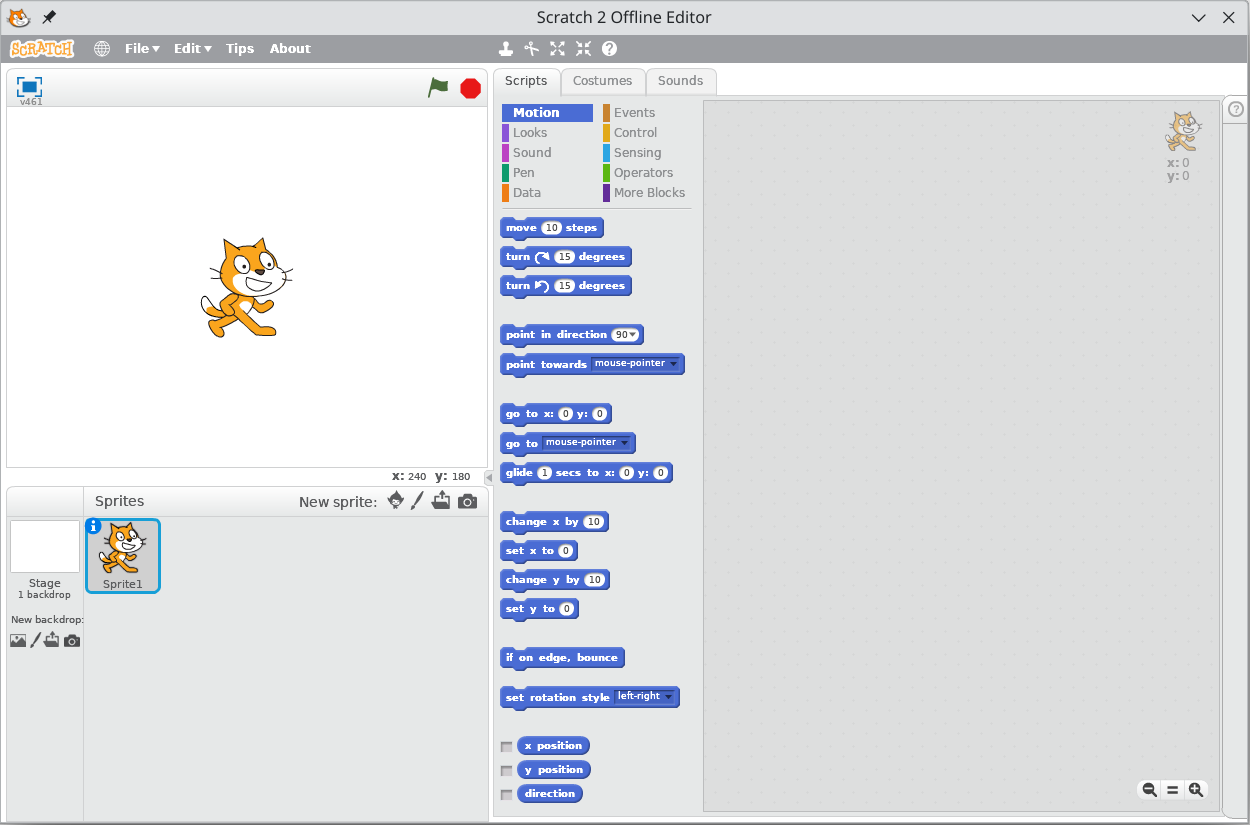
\includegraphics[width=\linewidth]{scratch-2}
    \end{wide}
    \caption{The Scratch 1.0 desktop application (top) and Scratch 2.0 offline editor (bottom).}
    \label{fig:scratch-1.0}
\end{figure}


The first public release of Scratch was in May 2007 as a desktop application (\cref{fig:scratch-1.0}), written in Squeak, a Smalltalk implementation.
This version already supported sharing projects by uploading them to the Scratch website.
Scratch 2.0, released in May 2013, was a rewrite providing the first ``online'' version of Scratch (running in the browser).
It used Adobe Flash for the online version and Adobe Air for the downloadable offline editor.

\marginnote{At the time, some users speculated that Scratch 3 was ``rushed'' since it was announced in 2017 that support for Flash would end in 2021. Work on Scratch 3, however, started in May 2016.}
In January 2019, Scratch 3.0 was released.
This version is a complete rewrite, using web technologies, such as JavaScript, HTML, and CSS\@.
Scratch 3.0 is fully browser-based but still supports an offline editor using Electron.\footnote{\url{https://scratch.mit.edu/download}}
Scratch 3.0 consists of a set of independent source code modules that work together to form the complete Scratch environment.
An overview of the relationships between the modules is shown in \cref{fig:scratch-dependencies}.
Each module is developed independently in a separate repository on GitHub.

% Ugly but what can you do
{
    %! suppress = Makeatletter
    \makeatletter
    \@beginparpenalty=10000
    %! suppress = Makeatletter
    \makeatother
    The most important and relevant modules for this dissertation are:

    \begin{description}
        \item[Scratch Blocks] A fork of Google's Blockly~\autocite{pasternakTipsCreatingBlock2017}, a library for building block-based computing interfaces.\footnote{\url{https://github.com/scratchfoundation/scratch-blocks}}
        \item[Scratch Virtual Machine] The runtime engine behind Scratch and responsible for running the projects created by the blocks.\footnote{\url{https://github.com/scratchfoundation/scratch-vm}}
        \item[Scratch User Interface] A React-based web application that consists of the Scratch programming environment.
        It uses and builds on the other components.\footnote{\url{https://github.com/scratchfoundation/scratch-gui}}
        \item[Scratch Renderer] A WebGL-based renderer, responsible for rendering the canvas.\footnote{\url{https://github.com/scratchfoundation/scratch-render}}
    \end{description}
}

\begin{figure}
    \begin{wide}
        \includestandalone[width=\linewidth]{dependencies}
    \end{wide}
    \caption{
        Overview of the dependencies between the Scratch repositories (using their repository name).
        The repositories that are purely for the hosted instance, such as the website, account system, and forum are left out.
        An arrow indicates a dependency.
        For example, the \texttt{scratch-gui} package has five dependencies.
    }
    \label{fig:scratch-dependencies}
\end{figure}

\end{document}
